% !TeX spellcheck = fr_FR
\thispagestyle{noheader}
\chapter*{Résumé} % No (numbered) toc entry with *

\tikz[remember picture,overlay] \node[shift={(4.165cm,-1.955cm)}]
	at (current page.north west)
	{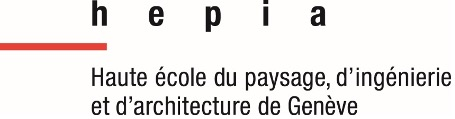
\includegraphics[height=1.29cm]{template/images/title/hepia_logo}};
	\tikz[remember picture,overlay] \node[shift={(-4.238cm,-1.97cm)}]
	at (current page.north east)
	{
\includegraphics[height=1.29cm]{template/images/title/hes-so_geneve_logo}};

\addcontentsline{toc}{chapter}{Résumé} % Adding toc entry
\thispagestyle{noheader}

\begin{spacing}{0.956}
\vspace{0.5cm}

La lumière Cherenkov est un phénomène physique similaire à un boom supersonique dans le domaine électromagnétique.
Lorsque des particules chargées entrent dans notre atmosphère à la vitesse de la lumière, 
elles démarrent une réaction en chaîne produisant une pluie de lumières atmosphérique.
L’observation de ces pluies nous permet de mieux comprendre les mécanismes de la physique de particules. 
Dans cette optique, l’UNIGE travaille sur la mission pionnière du satellite NUSES et du télescope spatial Terzina. 
Ce télescope a pour but de détecter et d’étudier les neutrinos de manière indirecte en observant le limbe de la terre 
et en y détectant des pluies de lumières atmosphériques de gamme d'énergie supérieure à 100PeV. 
Le but principal de ce projet est d'aider à pallier le problème technique de la bande passante disponible. 
À cause de ressources limitées à bord du satellite, Terzina n’aura qu'accès à 40 Gbit de transmission par jour et cela ne suffirait 
pas à transmettre tous les évènements détectés en une journée. La solution imaginée est de créer un réseau de neurones
capable d'aider à la décision d'évènements d'intérêt. Il a aussi été imaginé d'utiliser ce même réseau neuronal
pour compenser la dégradation des capteurs à bord. Lors de ce travail j'ai commencé par prendre en main les différents
simulateurs de données existants suivi de recherches pour comprendre le phénomène physique. 
Ensuite, j'ai utilisé ces simulateurs pour tester des réseaux de neurones convolutifs. 
Et pour finir j'ai établi une liste de tâches restantes pour prouver l'efficacité et l'utilité d'un tel réseau de neurones.

\vfill
\begin{center}
	{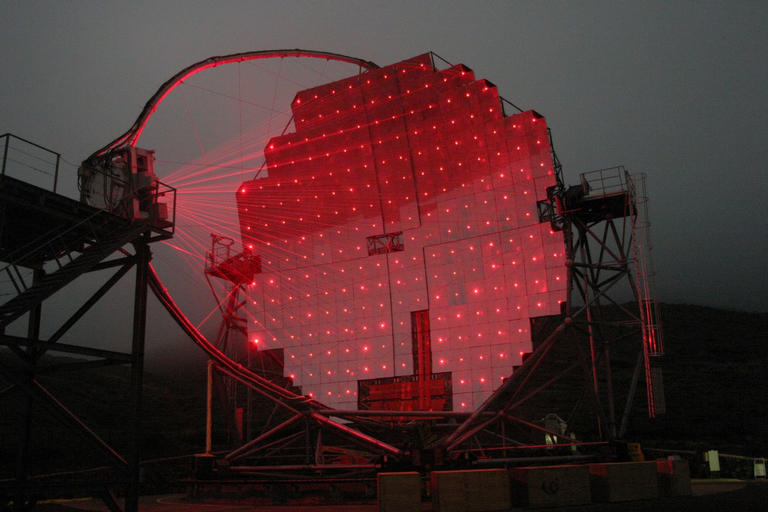
\includegraphics[width=0.4\linewidth]{MagicCalibration.jpg}}\\*
\vfill
%% CONTENT ENDS HERE

{
%%%%%%%%%%%%%%%%%%%%%%%%%%%%%%%%%%%%%%%%%%%%%%%%%%%%%%%%%%%%%%%%%%%%%%%%%%%%%%%%
%%%%%%%%%%%%%%%%%%%%%%%%%% DO NOT MODIFY THE TABLE BELOW %%%%%%%%%%%%%%%%%%%%%%%
%%%%%%%%%%%%%%%%%%%%%%%%%%%%%%%%%%%%%%%%%%%%%%%%%%%%%%%%%%%%%%%%%%%%%%%%%%%%%%%%
	\begin{tabular*}{16cm}{p{7.59cm} p{7.58cm}}
		\small Candidat-e:					&	\small Professeur-e(s) responsable(s):\\*[10pt]
		\small\textbf{\textsc{\Author}}		&	\small\textbf{\textsc{\Professor}}\\*[10pt]
		\footnotesize  Filière d’études : ISC	&	\footnotesize  \textbf{En collaboration avec:} UNIGE\\*[10pt]
		\footnotesize  {} & \footnotesize  Travail de bachelor soumis à une convention de stage en entreprise: \Convention\\*[20pt]
		\footnotesize  {} & \footnotesize  Travail soumis à un contrat de confidentialité: \Confidentiel\\*[10pt]
	\end{tabular*}\\*[1.9cm]
}
\end{center}
\end{spacing}
